\scanpage{57}
% E: text|printed header upper left|//* CRAY2 0296 I
\texttt{//*\quad CRAY2\quad 0296\qquad I}
% E: display|top handwritten calculation|nu(n-1)+nu(n-3)
\[
\nu(\underbrace{n-1}_{\unsure{2}})+\nu(n-3)=2\nu n-4\nu
\deleted{{}=2\nu(n-1)}\qquad\deleted{{}=\nu(2n-3)}
\]
\[=\boxed{2\nu(n-2)}\]
\[\unsure{2(n-2)}\]
% E: drawing|top right at torn corner|pentagon labelled 0 1 2 3 4
\figure{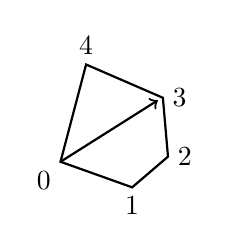
\begin{tikzpicture}[scale=.65]
\draw[thick] (0,0)--(1.4,-.5)--(2.1,.1)--(2,1.25)--(.5,1.9)--cycle;
\draw[->,thick] (0,0)--(1.9,1.2);
\node[below left] at (0,0) {$0$};\node[below] at (1.4,-.5) {$1$};\node[right] at (2.1,.1) {$2$};\node[right] at (2,1.25) {$3$};\node[above] at (.5,1.9) {$\unsure{4}$};
\end{tikzpicture}}
% E: drawing|printed upper banner|0051 formed from repeated digits
\figure{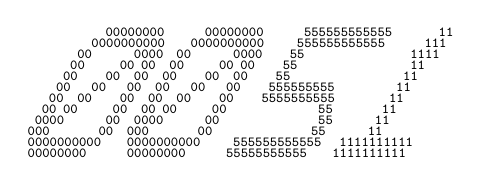
\begin{tikzpicture}[x=.09cm,y=.14cm,every node/.style={font=\tiny\ttfamily,anchor=west,inner sep=0pt}]
\foreach \d in {0,14}{
\node at ({\d+11},0) {00000000};\node at ({\d+9},-1) {0000000000};
\node at ({\d+7},-2) {00};\node at ({\d+15},-2) {0000};
\node at ({\d+6},-3) {00};\node at ({\d+13},-3) {00};\node at ({\d+16},-3) {00};
\node at ({\d+5},-4) {00};\node at ({\d+11},-4) {00};\node at ({\d+15},-4) {00};
\node at ({\d+4},-5) {00};\node at ({\d+9},-5) {00};\node at ({\d+14},-5) {00};
\node at ({\d+3},-6) {00};\node at ({\d+7},-6) {00};\node at ({\d+13},-6) {00};
\node at ({\d+2},-7) {00};\node at ({\d+5},-7) {00};\node at ({\d+12},-7) {00};
\node at ({\d+1},-8) {0000};\node at ({\d+11},-8) {00};
\node at (\d,-9) {000};\node at ({\d+10},-9) {00};
\node at (\d,-10) {0000000000};\node at (\d,-11) {00000000};}
\node at (39,0) {555555555555};\node at (38,-1) {555555555555};
\node at (37,-2) {55};\node at (36,-3) {55};\node at (35,-4) {55};
\node at (34,-5) {555555555};\node at (33,-6) {5555555555};
\node at (41,-7) {55};\node at (41,-8) {55};\node at (40,-9) {55};
\node at (29,-10) {555555555555};\node at (28,-11) {55555555555};
\node at (58,0) {11};\node at (56,-1) {111};\node at (54,-2) {1111};
\foreach \r in {3,4,5,6,7,8,9}{\node at ({57-\r},-\r) {11};}
\node at (44,-10) {1111111111};\node at (43,-11) {1111111111};
\end{tikzpicture}}
% E: drawing|upper left over the printed digits|narrow brown loops and strokes
\figure{
\begin{tikzpicture}[scale=.65]
\draw[brown!65!black,thin] (0,0)..controls (-.2,3.1) and (-.35,4.2)..(-.5,3.4)..controls (-.6,1.8) and (-.2,1.6)..(0,2.3)
(.6,.7)..controls (.4,3.6) and (.15,4.3)..(.1,3.8)..controls (.05,2.9) and (.4,1.7)..(.7,1.1)
(1.2,.1)..controls (.9,3.2) and (.9,2.8)..(.9,1.5)
(1.8,.1)..controls (1.4,4.6) and (1.1,4.8)..(1.2,3.4)..controls (1.4,1.1) and (1.9,-.5)..(2.1,-.7)
(2.5,.1)..controls (2.2,4.2) and (1.9,5.9)..(1.8,5.2)..controls (1.8,3.8) and (2.6,1.1)..(2.9,.15)
(3.8,0)..controls (3.7,.9) and (3.6,1.6)..(3.25,2.5);
\end{tikzpicture}}
% E: drawing|upper row left green polygon|inverted (3,5)
% E: drawing|upper row middle green polygon|inverted (3,4)
% E: drawing|upper row right green polygon|inverted (3,3)
% E: drawing|upper row separating line|vertical green line
\figure{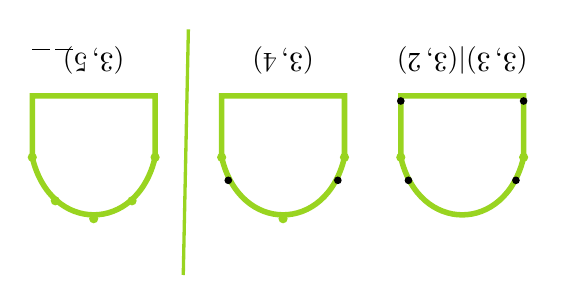
\begin{tikzpicture}[scale=.65]
\foreach \d in {0,3.7,7.2}{\draw[yellow!60!green,line width=2pt] (\d,2)--({\d+2.4},2)--({\d+2.4},.8)..controls ({\d+2.05},-.7) and ({\d+.35},-.7)..(\d,.8)--cycle;
\foreach \x/\y in {0/.8,2.4/.8}{\fill[yellow!60!green] ({\d+\x},\y) circle(.09);}}
\foreach \p in {(.45,-.05),(1.2,-.4),(1.95,-.05),(4.9,-.4)}{\fill[yellow!60!green] \p circle(.09);}
\foreach \p in {(3.83,.35),(5.97,.35),(7.2,1.9),(9.6,1.9),(7.35,.35),(9.45,.35)}{\fill \p circle(.075);}
\node[rotate=180] at (1.2,2.7) {$\unsure{(3,5)}$};\node[rotate=180] at (4.9,2.7) {$(3,4)$};\node[rotate=180] at (8.4,2.7) {$\unsure{(3,3)|(3,2)}$};
\draw[yellow!60!green,line width=1.2pt] (3.05,3.3)--(2.95,-1.5);
\draw (0,2.9)--(.35,2.9) (.45,2.9)--(.8,2.9);
\end{tikzpicture}}
% E: drawing|upper right below pentagon|diamond with arrow and numbered vertices
% E: drawing|upper right beside diamond|trapezoid thick lower edge
% E: drawing|right centre pencil oval|oval with lower label 1
\figure{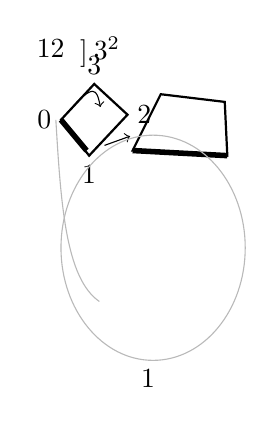
\begin{tikzpicture}[scale=.65]
\node at (-.2,2.1) {$\unsure{12}$};\node at (.45,2) {$\unsure{]}$};\node at (.9,2.1) {$\unsure{3^{2}}$};
\draw[thick] (0,.7)--(.65,1.4)--(1.3,.8)--(.55,0)--cycle;
\draw[line width=2pt] (0,.7)--(.5,.1);\draw[->] (.12,.83)..controls (.65,1.45) and (.7,1.3)..(.77,.95);
\draw[->] (.85,.2)--(1.35,.38);
\node[left] at (0,.7) {$0$};\node[below] at (.55,0) {$1$};\node[right] at (1.3,.8) {$2$};\node[above] at (.65,1.4) {$3$};
\draw[thick] (1.4,.1)--(1.95,1.2)--(3.2,1.05)--(3.25,0)--cycle;
\draw[line width=2pt] (1.4,.1)--(3.25,0);
\draw[gray!55] (1.8,-1.8) ellipse (1.8 and 2.2);
\draw[gray!55] (-.1,.7)..controls (.0,-1) and (.1,-2.4)..(.75,-2.85);
\node[below] at (1.7,-4) {$\unsure{1}$};
\end{tikzpicture}}
% E: drawing|middle left pair of green polygons|inverted (3,3) (3,4) and minus-one braces
\figure{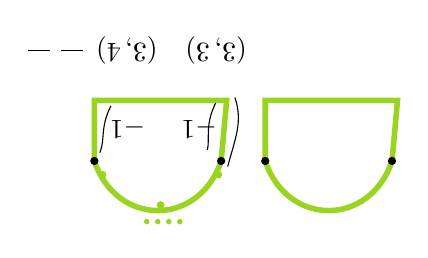
\begin{tikzpicture}[scale=.7]
\foreach \d in {0,3.1}{\draw[yellow!60!green,line width=2pt] (\d,2)--({\d+2.4},2)--({\d+2.3},.9)..controls ({\d+1.9},-.3) and ({\d+.4},-.3)..(\d,.9)--cycle;
\fill (\d,.9) circle(.075);\fill ({\d+2.3},.9) circle(.075);}
\foreach \p in {(.15,.65),(1.2,.1),(2.25,.65)}{\fill[yellow!60!green] \p circle(.07);}
\foreach \x in {.95,1.15,1.35,1.55}{\fill[yellow!60!green] (\x,-.2) circle(.05);}
\draw (2.55,2.05)..controls (2.7,1.6) and (2.55,1.3)..(2.42,.8);
\node[rotate=180] at (1.4,2.9) {$(3,3)\quad(3,4)$};
\node[rotate=180] at (.6,1.5) {$-1$};\node[rotate=180] at (1.9,1.5) {$-1$};
\draw (.3,1.9)..controls (.1,1.5) and (.2,1.3)..(.1,1.05) (2.2,1.95)..controls (2,1.55) and (2.1,1.3)..(2.05,1.1);
\draw (-.6,2.9)--(-.2,2.9) (-1.2,2.9)--(-.8,2.9);
\end{tikzpicture}}
% E: drawing|printed middle banner|CRAY2 formed from repeated characters
\figure{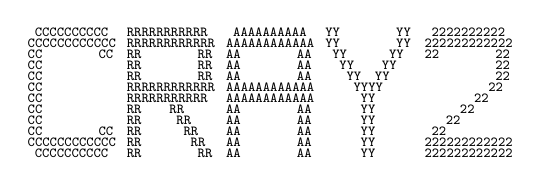
\begin{tikzpicture}[x=.09cm,y=.14cm,every node/.style={font=\tiny\ttfamily,anchor=west,inner sep=0pt}]
\node at (1,0) {CCCCCCCCCC}; \node at (0,-1) {CCCCCCCCCCCC};
\foreach \r in {2,3,4,5,6,7,8,9}{\node at (0,-\r) {CC};}
\node at (10,-2) {CC}; \node at (10,-9) {CC};
\node at (0,-10) {CCCCCCCCCCCC}; \node at (1,-11) {CCCCCCCCCC};
\node at (14,0) {RRRRRRRRRRR}; \node at (14,-1) {RRRRRRRRRRRR};
\foreach \r in {2,3,4,7,8,9,10,11}{\node at (14,-\r) {RR};}
\foreach \r in {2,3,4}{\node at (24,-\r) {RR};}
\node at (14,-5) {RRRRRRRRRRRR}; \node at (14,-6) {RRRRRRRRRRR};
\node at (20,-7) {RR}; \node at (21,-8) {RR}; \node at (22,-9) {RR}; \node at (23,-10) {RR}; \node at (24,-11) {RR};
\node at (29,0) {AAAAAAAAAA}; \node at (28,-1) {AAAAAAAAAAAA};
\foreach \r in {2,3,4,7,8,9,10,11}{\node at (28,-\r) {AA}; \node at (38,-\r) {AA};}
\node at (28,-5) {AAAAAAAAAAAA}; \node at (28,-6) {AAAAAAAAAAAA};
\foreach \r in {0,1}{\node at (42,-\r) {YY}; \node at (52,-\r) {YY};}
\node at (43,-2) {YY}; \node at (51,-2) {YY};
\node at (44,-3) {YY}; \node at (50,-3) {YY};
\node at (45,-4) {YY}; \node at (49,-4) {YY};
\node at (46,-5) {YYYY};
\foreach \r in {6,7,8,9,10,11}{\node at (47,-\r) {YY};}
\node at (57,0) {2222222222}; \node at (56,-1) {222222222222};
\node at (56,-2) {22}; \node at (66,-2) {22};
\node at (66,-3) {22}; \node at (66,-4) {22}; \node at (65,-5) {22}; \node at (63,-6) {22}; \node at (61,-7) {22}; \node at (59,-8) {22}; \node at (57,-9) {22};
\node at (56,-10) {222222222222}; \node at (56,-11) {222222222222};
\end{tikzpicture}}
% E: drawing|centre over listing|green circle with black arcs and red ticks
\figure{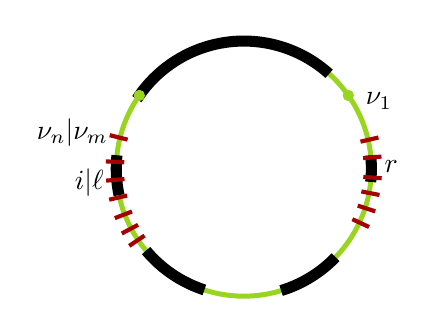
\begin{tikzpicture}[scale=.9]
\draw[yellow!60!green,line width=1.8pt] (0,0) circle(1.8);
\foreach \a/\b in {48/147,174/192,220/252,287/316,354/366}{\draw[line width=4pt] (\a:1.8) arc (\a:\b:1.8);}
\foreach \a in {145,35}{\fill[yellow!60!green] (\a:1.8) circle(.08);}
\foreach \a in {166,177,185,193,201,208,214,335,342,349,356,365,373}{\draw[red!65!black,line width=1.5pt] (\a:1.69)--(\a:1.95);}
\node[left] at (164:1.85) {$\unsure{\nu_n|\nu_m}$};\node[left] at (186:1.85) {$\unsure{i|\ell}$};
\node[right] at (31:1.85) {$\nu_1$};\node[right] at (1:1.85) {$\unsure{r}$};
\end{tikzpicture}}
% E: text|printed middle lower six lines|START JOB 296 CRAY2
\texttt{****A\quad START\quad JOB\quad 296\quad CRAY2\qquad ROOM\qquad 5.00.32 PM 17 AUG 82\quad R6.PR1\quad SYS JES2\quad JOB 296\quad START\quad A****}\par
\texttt{****A\quad START\quad JOB\quad 296\quad CRAY2\qquad ROOM\qquad 5.00.32 PM 17 AUG 82\quad R6.PR1\quad SYS JES2\quad JOB 296\quad START\quad A****}\par
\texttt{****A\quad START\quad JOB\quad 296\quad CRAY2\qquad ROOM\qquad 5.00.32 PM 17 AUG 82\quad R6.PR1\quad SYS JES2\quad JOB 296\quad START\quad A****}\par
\texttt{****A\quad START\quad JOB\quad 296\quad CRAY2\qquad ROOM\qquad 5.00.32 PM 17 AUG 82\quad R6.PR1\quad SYS JES2\quad JOB 296\quad START\quad A****}\par
\texttt{****A\quad START\quad JOB\quad 296\quad CRAY2\qquad ROOM\qquad 5.00.32 PM 17 AUG 82\quad R6.PR1\quad SYS JES2\quad JOB 296\quad START\quad A****}\par
\texttt{****A\quad START\quad JOB\quad 296\quad CRAY2\qquad ROOM\qquad 5.00.32 PM 17 AUG 82\quad R6.PR1\quad SYS JES2\quad JOB 296\quad START\quad A****}
% E: text|printed notice heading|DERNIERE MISE A JOUR
\texttt{DERNIERE MISE A JOUR DE JOURNAL : 11-08-82}\par
\texttt{ARRET DE L'ORDINATEUR LE MERCREDI 18 AOUT DE 7 H A 8 H.}\par
\texttt{ATTENTION .........}
% E: text|printed notice three lines|UN ARRET EXCEPTIONNEL
\texttt{1\qquad UN ARRET EXCEPTIONNEL POUR PREPARER L'ARRIVEE DE NOUVELLES}\par
\texttt{1\qquad UNITES AURA LIEU DU VENDREDI 20 AOUT A 17H 30 AU LUNDI}\par
\texttt{1\qquad 23 AOUT A 8H.}
% E: drawing|lower left|faint oval with dark upper and lower arcs
% E: drawing|lower left beside oval|long curved brown arrow
% E: drawing|lower middle|oval green vertices black arcs and narrow strip
% E: drawing|lower right|oval three black arcs two green vertices
% E: drawing|between lower middle and right|brown zigzag
\figure{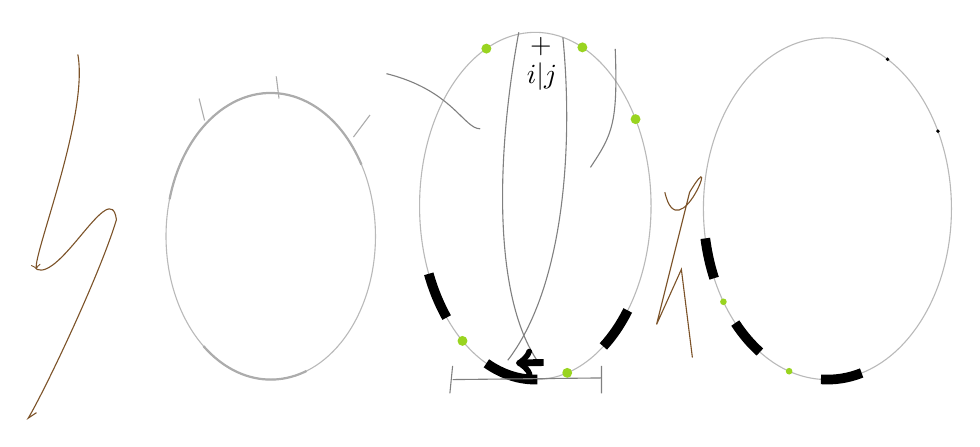
\begin{tikzpicture}[scale=.7]
\draw[gray!55] (0,0) ellipse (1.9 and 2.6);
\draw[gray!65,thick] (30:1.9 and 2.6) arc (30:165:1.9 and 2.6) (230:1.9 and 2.6) arc (230:290:1.9 and 2.6);
\draw[gray!65] (-1.2,2.1)--(-1.3,2.5) (.15,2.5)--(.1,2.9) (1.5,1.8)--(1.8,2.2);
\draw[brown!65!black,->] (-3.5,3.3)..controls (-3.3,2.2) and (-4.3,-.3)..(-4.25,-.6);
\draw[brown!65!black] (-4.25,-.6)..controls (-3.8,-.8) and (-2.9,1.1)..(-2.8,.3)..controls (-3.1,-.7) and (-4.1,-2.8)..(-4.4,-3.3)--(-4.25,-3.2);
\begin{scope}[shift={(4.8,.55)}]
\draw[gray!55] (0,0) ellipse (2.1 and 3.15);
\foreach \a in {30,66,115,231,286}{\fill[yellow!60!green] (\a:2.1 and 3.15) circle(.09);}
\foreach \a/\b in {203/220,245/271,306/323}{\draw[line width=3.5pt] (\a:2.1 and 3.15) arc (\a:\b:2.1 and 3.15);}
\draw[gray] (-.3,3.15)..controls (-.7,1) and (-.8,-1.7)..(.1,-2.9);
\draw[gray] (.5,3.06)..controls (.7,1) and (.5,-1.5)..(-.5,-2.8);
\draw[gray] (-2.7,2.4)..controls (-1.5,2.1) and (-1.3,1.4)..(-1,1.4);
\draw[gray] (1.45,2.85)..controls (1.5,1.5) and (1.4,1.3)..(1.0,.7);
\draw[gray] (-1.5,-3.15)--(1.2,-3.12) (-1.55,-3.4)--(-1.5,-2.9) (1.2,-3.4)--(1.2,-2.9);
\draw[<-,line width=2.5pt] (-.35,-2.85)--(.15,-2.84);
\node at (.1,2.9) {$+$};\node at (.12,2.35) {$\unsure{i|j}$};
\end{scope}
\begin{scope}[shift={(10.1,.5)}]
\draw[gray!55] (0,0) ellipse (2.25 and 3.1);
\foreach \a/\b in {190/204,222/237,267/286}{\draw[line width=3.5pt] (\a:2.25 and 3.1) arc (\a:\b:2.25 and 3.1);}
\foreach \a in {213,252}{\fill[yellow!60!green] (\a:2.25 and 3.1) circle(.06);}
\fill (61:2.25 and 3.1) circle(.035) (27:2.25 and 3.1) circle(.035);
\draw[brown!65!black] (-2.95,.3)..controls (-2.7,-.8) and (-1.9,1.3)..(-2.5,.3)--(-3.1,-2.1)--(-2.65,-1.1)--(-2.45,-2.7);
\end{scope}
\end{tikzpicture}}
\mspage{56}
